\section{AirQuality}\label{sec:AirQuality}

O número grupo é par, por isso, um dos conjunto de dados atribuídos foi o \emph{AirQuality}.
Este dataset contém 9358 instâncias de respostas médias horárias de uma matriz de 5 sensores químicos de óxido metálico dentro de um dispositivo multi-sensor químico de qualidade do ar. O dispositivo estava localizado numa área significativamente poluída, ao nível da estrada, dentro de uma cidade italiana. Os dados foram registados de março de 2004 a fevereiro de 2005 (um ano). A cada hora são registadas as concentrações médias de CO, Hidrocarbonetos Não Metánicos, Benzeno, Óxidos de Nitrogénio Total (NOx) e Dióxido de Nitrogénio (NO2) fornecidos por um analisador certificado de referência co-localizado. Contém 15 atributos e os valores em falta são representados por -200.

\subsection{Objetivos do estudo}

Uma das primeiras coisas que o grupo detetou neste conjunto de dados foi a presença de valores nulos em grande quantidade, indicando que ou o valor registado pelo sensor em questão não é válido (por exemplo má calibração do sensor) ou o valor simplesmente não foi registado. Este foi o ponto de partida para o nosso estudo, uma vez que definimos como um dos objetivos encontrar um modelo de Regressão Linear que nos permitisse estimar os valores em falta, não só para os dados presentes no conjunto como para eventuais falhas futuras.
Por outro lado, achamos também pertinente tentar perceber de que maneira os poluentes no ar se relacionam entre si, para assim entender, por exemplo, formas efetivas de colmatar o problema. Para isto vai ser usado um modelo de Associação que permite estabelecer relações entre os diferentes atributos.

\subsection{Atributos do conjunto de dados}

De seguida listam-se os atributos originais do conjunto de dados e a sua descrição.

\begin{table}
\centering
\label{airqualitytable}
\resizebox{\textwidth}{!}{\begin{tabular}{|l|l|l|}
\hline
Atributo             & Descrição                                    & Tipo           \\ \hline
Date                 & Data do registo                             & Date           \\ \hline
Time                 & Hora do registo                             & Date           \\ \hline
Concentração de CO\footnote{Monóxido de Carbono}   & Concentração média de CO em mg/metro3       & Valor numérico \\ \hline
PT08.S1(CO)          & Resposta média do sensor 1 por hora         & Valor numérico \\ \hline
Concentração de NMHC\footnote{Hidrocarbonetos não metánicos} & Concentração média de NMHC em microg/metro3 & Valor numérico \\ \hline
Concentração de C6H6 & Concentração média de C6H6 em microg/metro3 & Valor numérico \\ \hline
PT08.S2(NMHC)        & Resposta média do sensor 2 por hora         & Valor numérico \\ \hline
Concentração de NOx\footnote{Óxidos de nitrogénio}  & Concentração média de Nox em ppb            & Valor numérico \\ \hline
PT08.S3(NOx)        & Resposta média do sensor 3 por hora         & Valor numérico \\ \hline
NO2\footnote{Dióxido de Nitrogénio}       & Concentração média de NO2 em ppb         & Valor numérico \\ \hline
PT08.S4(NO2)        & Resposta média do sensor 4 por hora         & Valor numérico \\ \hline
PT08.S5(O3)        & Resposta média do sensor 5 por hora         & Valor numérico \\ \hline
T        & Temperatura em graus Celsius         & Valor numérico \\ \hline
RH       & Percentagem de humidade relativa         & Valor numérico \\ \hline
AH      & Humidade Absoluta         & Valor numérico \\ \hline
\end{tabular}}
\end{table}

Pela primeira análise aos atributos conseguimos facilmente perceber que o conjunto de dados é de bastante valor um vez que temos todos os atributos de valor numérico e, por isso, facilmente analisados.
\newpage
\subsection{Preparação do conjunto}

Para uma posterior correta análise dos dados foi necessário , antes de partir para a exploração dos dados, tratar os dados tendo em vista a sua uniformização. Para isso foram utilizadas duas ferramentas: Excel e o Weka.

O primeiro passo neste conjunto de dados foi separar a data para ser possível retirar conclusões quanto a dias, meses e anos em separado. Para isso dividiu-se o atributo Date em três novos atributos: Day, Month e Year.

\begin{figure}[H]
    \centering
    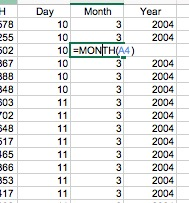
\includegraphics[scale=1]{tex/img/img1.jpg}
    \caption{Fórmula utilizada no Excel}
    \label{fig:Novos Atributos}
\end{figure}


Um dos primeiros problemas detetados pelo grupo neste dataset foi a presença de valores nulos identificados com o valor -200. Como o Weka interpreta isso como mais um valor do dataset e não como um valor nulo todos estes valores foram alterados para ?. Foi também necessário alterar os field separator e line separator do ficheiro .csv.
De seguida dividiu-se o problema em duas instâncias. A primeira instância seria aquela à qual se iria aplicar Regressão Linear e para isso foi necessário o seguinte conjunto de passos:

\begin{enumerate}
	\item Transformar o separador decimal em ponto
	\item Retirar o line separator do \.csv
	\item Transformar o atribute separator para vírgula.
	\item Carregar os dados para o Weka e remover os atributos relacionados com o tempo já que pretendiamos um modelo onde o tempo e a hora não fosse influência dos restantes fatores
	\item Passar os atributos do tipo String para Nominal e através da edição do ficheiro .arff mudar para numeric
\end{enumerate}

A segunda instância seria aquela onde se iria aplicar métodos de Associação e para isso foi necessário o seguinte conjunto de passos:

\begin{enumerate}
	\item Passar o atributo Time para Hour uma vez que todas as horas representadas eram absolutas, passando este a ser um atributo do tipo numérico
	\item Transformar o separador decimal em ponto
	\item Retirar o line separator do \.csv
	\item Transformar o atribute separator para \,
	\item Carregar os dados para o Weka 
	\item Passar os atributos do tipo String para Nominal
	\item Aplicar o filtro Discretize aos dados Nominal
	\item Remover os atributos Year e Month
\end{enumerate}


\begin{figure}[H]
    \centering
    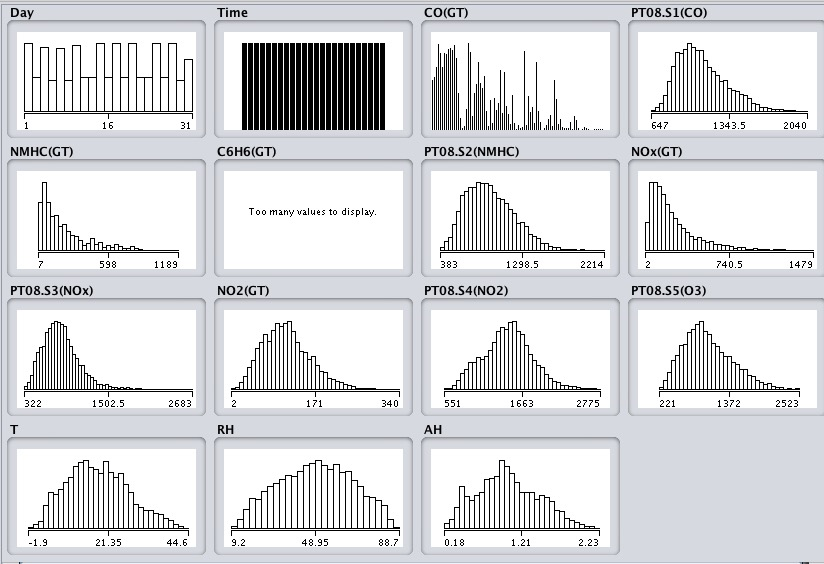
\includegraphics[scale=0.4]{tex/img/img2.jpg}
    \caption{AirQuality - conjunto de dados para regressão}
    \label{fig:regressao}
\end{figure}

\begin{figure}[H]
    \centering
    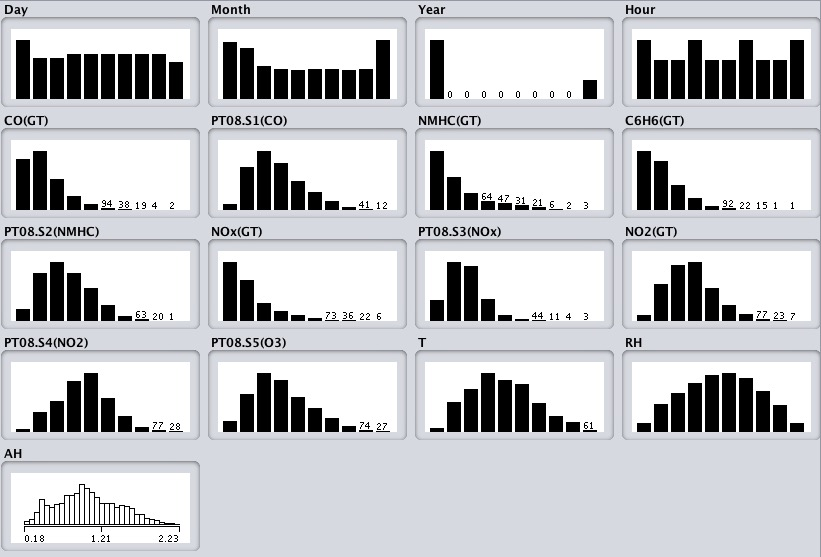
\includegraphics[scale=0.4]{tex/img/img3.jpg}
    \caption{AirQuality - conjunto de dados para associação}
    \label{fig:associacao}
\end{figure}

\newpage

\subsection{Regressão linear}

Utilizou-se o classificador de Regressão Linear do Weka para estimar os diversos atributos através dos restantes. Para isto as configurações definidas foram o algoritmo M5 eliminando os atributos co-lineares.

\textbf{Função estimada pela regressão para calcular o atributo CO(GT)}

\begin{lstlisting}[frame=single]

=== Classifier model (full training set) ===


Linear Regression Model

CO(GT) =

      0.0013 * PT08.S1(CO) +
      0.001  * NMHC(GT) +
      0.0822 * C6H6(GT) +
      0.0025 * NOx(GT) +
      0.0002 * PT08.S3(NOx) +
      0.0022 * NO2(GT) +
      0.0011 * PT08.S4(NO2) +
     -0.0005 * PT08.S5(O3) +
     -0.0226 * T +
     -0.0069 * RH +
     -0.0853 * AH +
     -1.6358

Time taken to build model: 0.07 seconds

=== Evaluation on training set ===

Time taken to test model on training data: 0.07 seconds

=== Summary ===

Correlation coefficient                  0.9427
Mean absolute error                      0.3077
Root mean squared error                  0.4847
Relative absolute error                 27.5315 %
Root relative squared error             33.352  %
Total Number of Instances             7674     
Ignored Class Unknown Instances               1683     

\end{lstlisting}
\newpage


\noindent
\textbf{Função estimada pela regressão para calcular o atributo NMHC(GT)}

\begin{lstlisting}[frame=single]

Linear Regression Model

NMHC(GT) =

     88.4515 * CO(GT) +
     -0.507  * PT08.S1(CO) +
      0.625  * PT08.S2(NMHC) +
      0.0798 * PT08.S3(NOx) +
      0.1362 * PT08.S4(NO2) +
     -0.0317 * PT08.S5(O3) +
     -9.5206 * T +
     -3.5289 * RH +
    247.2342 * AH +
   -116.041 

Time taken to build model: 0.01 seconds

=== Evaluation on training set ===

Time taken to test model on training data: 0.06 seconds

=== Summary ===

Correlation coefficient                  0.9125
Mean absolute error                     61.9972
Root mean squared error                 83.5736
Relative absolute error                 39.6808 %
Root relative squared error             40.8977 %
Total Number of Instances              914     
Ignored Class Unknown Instances               8443       

\end{lstlisting}


\newpage


\textbf{Função estimada pela regressão para calcular o atributo C6H6(GT)}

\begin{lstlisting}[frame=single]

=== Classifier model (full training set) ===


Linear Regression Model

C6H6(GT) =

      0.2704 * CO(GT) +
      0.001  * PT08.S1(CO) +
      0.0016 * NMHC(GT) +
      0.028  * PT08.S2(NMHC) +
      0.0031 * NOx(GT) +
      0.0037 * PT08.S3(NOx) +
     -0.0103 * NO2(GT) +
      0.0005 * PT08.S4(NO2) +
     -0.0003 * PT08.S5(O3) +
     -0.0963 * T +
     -0.0276 * RH +
      1.2435 * AH +
    -19.5928

Time taken to build model: 0.04 seconds

=== Evaluation on training set ===

Time taken to test model on training data: 0.05 seconds

=== Summary ===

Correlation coefficient                  0.9883
Mean absolute error                      0.8159
Root mean squared error                  1.138 
Relative absolute error                 14.1102 %
Root relative squared error             15.277  %
Total Number of Instances             8991     
Ignored Class Unknown Instances                366     

\end{lstlisting}


\newpage

\noindent
\textbf{Função estimada pela regressão para calcular o atributo NMHC(GT)}

\begin{lstlisting}[frame=single]

=== Classifier model (full training set) ===


Linear Regression Model

PT08.S2(NMHC) =

     -2.3276 * CO(GT) +
     -0.0412 * NMHC(GT) +
     23.8649 * C6H6(GT) +
      0.0163 * NOx(GT) +
     -0.1706 * PT08.S3(NOx) +
      0.1317 * NO2(GT) +
      0.1318 * PT08.S4(NO2) +
      0.0477 * PT08.S5(O3) +
      2.2441 * T +
    -76.4193 * AH +
    632.8796

Time taken to build model: 0.04 seconds

=== Evaluation on training set ===

Time taken to test model on training data: 1.29 seconds

=== Summary ===

Correlation coefficient                  0.9922
Mean absolute error                     24.4286
Root mean squared error                 33.1979
Relative absolute error                 11.3125 %
Root relative squared error             12.4422 %
Total Number of Instances             8991     
Ignored Class Unknown Instances                366  

\end{lstlisting}

\newpage


\textbf{Função estimada pela regressão para calcular o atributo NOx(GT)}

\begin{lstlisting}[frame=single]

=== Classifier model (full training set) ===


Linear Regression Model

NOx(GT) =

     64.8127 * CO(GT) +
     -0.0461 * PT08.S1(CO) +
     -0.2584 * NMHC(GT) +
     12.2255 * C6H6(GT) +
      0.2433 * PT08.S2(NMHC) +
      0.071  * PT08.S3(NOx) +
      1.2564 * NO2(GT) +
     -0.492  * PT08.S4(NO2) +
      0.0685 * PT08.S5(O3) +
      3.3026 * T +
      3.2582 * RH +
    104.3763 * AH +
    -24.4399

Time taken to build model: 0.04 seconds

=== Evaluation on training set ===

Time taken to test model on training data: 0.03 seconds

=== Summary ===

Correlation coefficient                  0.9246
Mean absolute error                     57.5821
Root mean squared error                 81.1059
Relative absolute error                 36.2008 %
Root relative squared error             38.0841 %
Total Number of Instances             7718     
Ignored Class Unknown Instances               1639   

\end{lstlisting}

\newpage

\textbf{Função estimada pela regressão para calcular o atributo NO2(GT)}

\begin{lstlisting}[frame=single]

=== Classifier model (full training set) ===


Linear Regression Model

NO2(GT) =

      5.6621 * CO(GT) +
      0.0219 * PT08.S1(CO) +
     -5.0209 * C6H6(GT) +
      0.1107 * PT08.S2(NMHC) +
      0.0997 * NOx(GT) +
     -0.0472 * PT08.S3(NOx) +
      0.0149 * PT08.S5(O3) +
     -0.5216 * RH +
    -36.8543 * AH +
     83.9743

Time taken to build model: 0.05 seconds

=== Evaluation on training set ===

Time taken to test model on training data: 0.05 seconds

=== Summary ===

Correlation coefficient                  0.8821
Mean absolute error                     16.9002
Root mean squared error                 22.786 
Relative absolute error                 44.2808 %
Root relative squared error             47.1107 %
Total Number of Instances             7715     
Ignored Class Unknown Instances               1642  

\end{lstlisting}


\newpage

\textbf{Função estimada pela regressão para calcular o atributo T}

\begin{lstlisting}[frame=single]

=== Classifier model (full training set) ===


Linear Regression Model

T =

     -0.1851 * CO(GT) +
     -0.0006 * NMHC(GT) +
     -0.3977 * C6H6(GT) +
      0.0107 * PT08.S2(NMHC) +
      0.0029 * NOx(GT) +
      0.0004 * PT08.S3(NOx) +
     -0.0018 * NO2(GT) +
      0.0058 * PT08.S4(NO2) +
     -0.0028 * PT08.S5(O3) +
     -0.3396 * RH +
     13.9848 * AH +
      8.6789

Time taken to build model: 0.04 seconds

=== Evaluation on training set ===

Time taken to test model on training data: 0.04 seconds

=== Summary ===

Correlation coefficient                  0.965 
Mean absolute error                      1.7173
Root mean squared error                  2.3153
Relative absolute error                 23.7038 %
Root relative squared error             26.2166 %
Total Number of Instances             8991     
Ignored Class Unknown Instances                366     

\end{lstlisting}


\newpage

\textbf{Função estimada pela regressão para calcular o atributo RH}

\begin{lstlisting}[frame=single]

=== Classifier model (full training set) ===


Linear Regression Model

RH =

     -0.3998 * CO(GT) +
      0.0095 * PT08.S1(CO) +
     -0.002  * NMHC(GT) +
     -0.772  * C6H6(GT) +
     -0.0008 * PT08.S2(NMHC) +
      0.0187 * NOx(GT) +
     -0.0018 * PT08.S3(NOx) +
     -0.0405 * NO2(GT) +
      0.0159 * PT08.S4(NO2) +
     -0.0015 * PT08.S5(O3) +
     -2.2981 * T +
     33.2042 * AH +
     36.6834

Time taken to build model: 0.05 seconds

=== Evaluation on training set ===

Time taken to test model on training data: 0.04 seconds

=== Summary ===

Correlation coefficient                  0.9376
Mean absolute error                      4.6628
Root mean squared error                  6.0204
Relative absolute error                 32.3253 %
Root relative squared error             34.7681 %
Total Number of Instances             8991     
Ignored Class Unknown Instances                366       

\end{lstlisting}

\newpage

\textbf{Função estimada pela regressão para calcular o atributo AH}

\begin{lstlisting}[frame=single]

=== Classifier model (full training set) ===


Linear Regression Model

AH =

     -0.0098 * CO(GT) +
     -0.0002 * PT08.S1(CO) +
      0.0147 * C6H6(GT) +
     -0.001  * PT08.S2(NMHC) +
      0.0002 * NOx(GT) +
     -0.0004 * PT08.S3(NOx) +
     -0.0009 * NO2(GT) +
      0.0005 * PT08.S4(NO2) +
      0.0001 * PT08.S5(O3) +
      0.0401 * T +
      0.0141 * RH +
      0.3426

Time taken to build model: 0.05 seconds

=== Evaluation on training set ===

Time taken to test model on training data: 0.01 seconds

=== Summary ===

Correlation coefficient                  0.9518
Mean absolute error                      0.095 
Root mean squared error                  0.1239
Relative absolute error                 28.9207 %
Root relative squared error             30.6792 %
Total Number of Instances             8991     
Ignored Class Unknown Instances                366  

\end{lstlisting}


Não aplicamos o modelo de regressão linear aos atributos PT08.Sx uma vez que entendemos que estes representavam características dos sensores e por isso não deveriam ser abrangidas pelo modelo.


\subsection{Associação}

Foi de seguida aplicado um algoritmo de Associação para retirar conhecimento a partir dos dados. O algoritmo utilizado foi o Apriori com as seguintes especificações:


\begin{figure}[H]
    \centering
    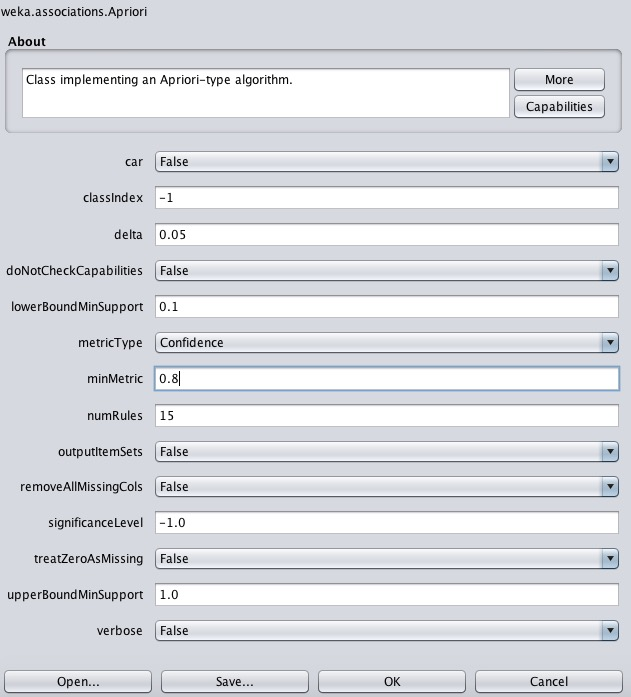
\includegraphics[scale=0.5]{tex/img/img5.jpg}
    \caption{Filtro Apriori}
    \label{fig:filtro}
\end{figure}

\newpage
\begin{lstlisting}[breaklines,frame=single]

Apriori
=======

Minimum support: 0.1 (936 instances)
Minimum metric <confidence>: 0.65
Number of cycles performed: 18

Generated sets of large itemsets:

Size of set of large itemsets L(1): 48

Size of set of large itemsets L(2): 24

Best rules found:

 1. NO2(GT)='(35.8-69.6]' 1298 ==> NOx(GT)='(-inf-149.7]' 1192    <conf:(0.92)> lift:(2.65) lev:(0.08) [741] conv:(7.92)
 2. PT08.S5(O3)='(1141.8-1372]' 1298 ==> PT08.S3(NOx)='(558.1-794.2]' 1015    <conf:(0.78)> lift:(2.28) lev:(0.06) [570] conv:(3.01)
 3. PT08.S1(CO)='(1064.9-1204.2]' 1951 ==> PT08.S3(NOx)='(558.1-794.2]' 1435    <conf:(0.74)> lift:(2.15) lev:(0.08) [766] conv:(2.48)
 4. NO2(GT)='(69.6-103.4]' 2001 ==> NOx(GT)='(-inf-149.7]' 1348    <conf:(0.67)> lift:(1.94) lev:(0.07) [654] conv:(2)

\end{lstlisting}
De referir que depois de algumas tentativas só conseguimos obter quatro regras para os dados, contudo tivemos que baixar o grau de confiança para \textgreater 65 \% .

\begin{itemize}
	\item Sempre que o valor de NO2 está entre 35.8 e 69.6 então o valor de NOx é sempre inferior a 149.7, com um grau de confiança de 92\%. 
	\item Sempre que o valor do sensor PT08.S5 está entre 1141.8 e 1372 então o valor do sensor PT08.S3(NOx) está entre 558.1 e 794.2, com um grau de confiança de 78\%.
	\item Sempre que o valor do sensor PT08.S1(CO) está entre 1064.9 e 1204.2 então o valor do sensor PT08.S3(NOx) está entre 558.1 e 794.2, com um grau de confiança de 74\%.
\end{itemize}

\subsection{Resultados e Recomendações}


Conseguimos assim obter os resultados pretendidos, de modo a obter funções de regressão linear que de maneira simples permitem estimar a grande quantidade de valores em falta no conjunto de dados. Foi também possível obter as regras de associação entre os diferentes atributos.
Da análise dos resultados obtidos tiramos as seguintes recomendações:

\begin{itemize}
	\item É possível diminuir a quantidade de tipos de medições já que alguns dos parâmetros são possíveis de ser estimados, ou seja, poderemos ter sensores de menor custo já que a quantidade de elementos a medir será menor;
	\item Com sensores de menor custo poderemos abranger mais área, permitindo perceber a poluição atmosférica de por exemplo uma cidade inteira;
	\item Sempre que a quantidade de Dióxido de Nitrogénio no ar está entre 35.8 e 69.6 então a quantidade de Óxido de Nitrogénio tem um máximo de 149.7, indicando que a libertação deste tipo de gases poluentes está relacionada;
	\item Sempre que os valores do sensor PT08.S1, calibrado para CO, está entre 1064.9 e 1204.2 então o valor do sensor PT08.S3, calibrado para NOx, está entre 558.1 e 794.2 indicando que as medições estão relacionadas.
\end{itemize}